\documentclass{article}

% if you need to pass options to natbib, use, e.g.:
% \PassOptionsToPackage{numbers, compress}{natbib}
% before loading nips_2016
%
% to avoid loading the natbib package, add option nonatbib:
% \usepackage[nonatbib]{nips_2016}

% \usepackage{nips_2016}

% to compile a camera-ready version, add the [final] option, e.g.:
\usepackage[final]{nips_2016}
\usepackage{graphicx}
\usepackage{caption}
\usepackage{subcaption}
\usepackage{amssymb,mathtools}

\usepackage[utf8]{inputenc} % allow utf-8 input
\usepackage[T1]{fontenc}    % use 8-bit T1 fonts
\usepackage{hyperref}       % hyperlinks
\usepackage{url}            % simple URL typesetting
\usepackage{booktabs}       % professional-quality tables
\usepackage{amsfonts}       % blackboard math symbols
\usepackage{nicefrac}       % compact symbols for 1/2, etc.
\usepackage{microtype}      % microtypography


\title{Reinforcement Learning for Chatbot with Emotions}

% The \author macro works with any number of authors. There are two
% commands used to separate the names and addresses of multiple
% authors: \And and \AND.
%
% Using \And between authors leaves it to LaTeX to determine where to
% break the lines. Using \AND forces a line break at that point. So,
% if LaTeX puts 3 of 4 authors names on the first line, and the last
% on the second line, try using \AND instead of \And before the third
% author name.

\author{
  Luyi Ma \\
  School of Computer Science\\
  Carnegie Mellon University\\
  Pittsburgh, PA 15213 \\
  \texttt{luyim@andrew.cmu.edu} \\
  \And
  Zhefan Zhu \\
  School of Computer Science \\
  Carnegie Mellon University\\
  Pittsburgh, PA 15213 \\
  \texttt{zhefanz@andrew.cmu.edu} \\  
  %% examples of more authors
  %% \And
  %% Coauthor \\
  %% Affiliation \\
  %% Address \\
  %% \texttt{email} \\
  %% \AND
  %% Coauthor \\
  %% Affiliation \\
  %% Address \\
  %% \texttt{email} \\
  %% \And
  %% Coauthor \\
  %% Affiliation \\
  %% Address \\
  %% \texttt{email} \\
  %% \And
  %% Coauthor \\
  %% Affiliation \\
  %% Address \\
  %% \texttt{email} \\
}

\begin{document}
% \nipsfinalcopy is no longer used

\maketitle



\section{Introduction}
In daily conversations, like on-line chatting, users send messages with emotional interactions instead of simple Q\&A pattern. A natural, fluent one-to-one conversation, generally, contains dialogues in which both users share similar emotion levels, such as happy, sadness. Our goal is to model a natural dialogue and the model can figure out users' emotions and response words with proper emotions.


\section{Background}

Dialogue systems, such as chatbots have become ubiquitous in modern society. A lot of chatbots have been presented so far. One of the latest chatbots is MILABOT, which is based on deep reinforcement learning, and developed by the Montreal Institute for Learning Algorithms (Serban, Sankar et al. 2017). Figure \ref{fig:dialoguesystem} shows their system control flow. In their chatbot, they have several response models to generate response separately to the input sentence, and the system is also given the dialogue history. The responses generated by sub-models are selected and evaluated according to some selection policies, and the best response is returned to the user. \par 





\begin{figure}[!h]
\begin{center}
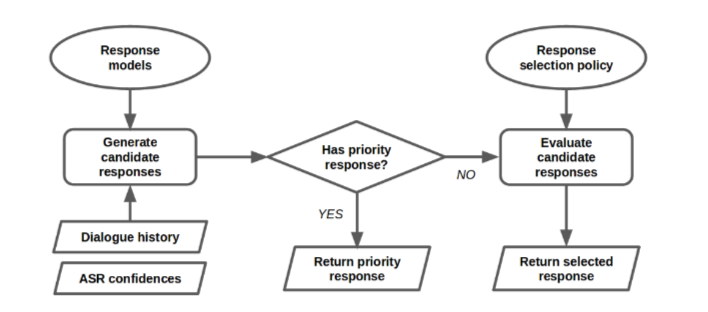
\includegraphics[scale=0.4]{figure1.png}
\caption{Dialogue manager control flow.}
\label{fig:dialoguesystem}
\end{center}
\end{figure}


The essential part of a dialogue system is response models. Common response models include knowledge based Q\&A systems, template based models, retrieval based neural networks, and generation based neural networks. \par



For our goal setting, we mainly focus on generation based neural networks. One typical model is the encoder-decoder framework of seq2seq model (Zhou, et al. 2017), where both layers are GRU layers (cho et al. 2014). In this framework, the encoder layer converts input sequence $X = (x_1, x_2, ..., x_n)$ to hidden state $h = (h_1, h_2, ..., h_n)$. And for the decoder layer, it takes in a context vector and previously decoded word to generate its state $s_t$. The output token is generated by sampling from the output probability distribution computed by $s_t$.




\section{Data and Method}

\subsection{Dataset and Preprocessing}

To train the response model, we collected 2.7 million sentences of subtitles from open subtitle database (\url{http://opus.lingfil.uu.se/OpenSubtitles.php/}). We choose subtitle dataset, because it is difficult to obtain chatting dataset, and subtitles are pretty similar to dialogues at most of the time. The subtitles of movies and TV programs provide sufficient conversation contents for training. Nevertheless, subtitles are slightly different from daily conversation due to theatrical and dramatic contents. We parsed conversations from original data which was in $.xml$ format, and filtered long segment of words which is impractical in daily conversation, which could be monologues in movies. \par

To train the model determining the emotion of a sentence, we used a dataset of tweets with emotion labels from http://knoesis.org/library/resource.php?id=1749 (Wang et al. 2012). This dataset tags tweets with seven emotions: anger, fear, joy, love, sadness, surprise and thankfulness. The format of the original dataset is: tweetId TAB emotionTag. We implemented a crawler to query tweet content from websites and constructed the training set. \par 

In addition, the word2seq embedding vectors (50 dimensions) are obtained from GloVe (https://nlp.stanford.edu/projects/glove/), which is used to transform words into vectors. 

\subsection{Long Short Term Memory (LSTM) and Seq2Seq Model}
In our task, we use Long Short Term Memory model (LSTM) as a building block to construct more complicated Sequence to Sequence model (Seq2Seq Model). The basic LSTM model is usually used for parsing sequential data. Lets say we have a sequence of inputs $x_1, x_2, ..., x_T \in \mathcal{R}^{m}$. With an initial cell state $c_0 = \mathbf{0} \in \mathcal{R}^{h}$ and an initial output $h_0 = \mathbf{0} \in \mathcal{R}^{h}$, inputs can be parsed by LSTM model with $h$ hidden units. At time $t \in [1, T]$, LSTM model does the following updates:
\begin{align*}
i_t &= \sigma(x_{t}^{T}W_i + h_{t-1}^{T}U_i + b_i)\\
f_t &= \sigma(x_{t}^{T}W_f + h_{t-1}^{T}U_f + b_f)\\
o_t &= \sigma(x_{t}^{T}W_o + h_{t-1}^{T}U_o + b_o)\\
\hat c_t &= \tanh(x_{t}^{T}W_c + h_{t-1}^{T}U_c + b_c)\\
c_t &= f_t \odot c_{t-1} + i_t \odot \hat c_t\\
h_t &= o_t \odot \tanh(c_t)
\end{align*}
, where $\sigma(\cdot)$ is the sigmoid function (element-wise) and $\odot$ is the element-wise product.

For the Seq2Seq recipe in our task, we adapt the multilayer LSTM model 
from Vinyals et al.[5]. Figure \ref{fig:LSTM_A} shows the multilayer LSTM model. $LSTM_{in}^{i}$ indicates the $i$-th encoding LSTM layer and $LSTM_{out}^{i}$ indicates the $i$-th decoding LSTM layer.
\begin{figure}[h]
	\centering
	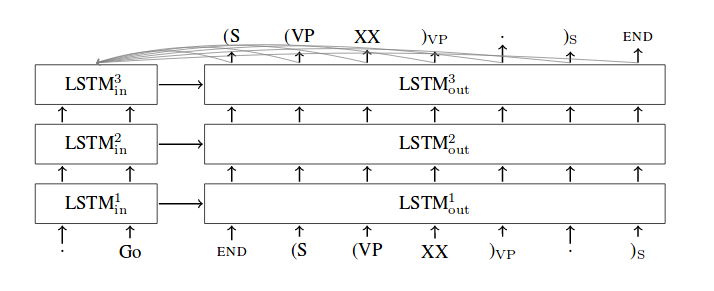
\includegraphics[width=0.7\linewidth]{LSTM_A}
	\caption{}
	\label{fig:LSTM_A}
\end{figure}

\subsection{Emotion in dialogue utterances}
Our task is to build a chatbot with the ability of considering the emotion of the utterances and react with a proper emotion. To extract or predict the emotion/mood of utterances, we use an one layer LSTM model to parse sentences and predict the type of emotions. Basically, we take the last hidden state, $h_T$, of the LSTM model for emotion classification:
\begin{align*}
O &= h_T^TW_1 + b_1\\
p &= SoftMax(O)\\
loss &= \frac{1}{N_{c}}\sum (y_i\log(p_i) + (1-y_i)\log(1 - p_i))
\end{align*}
, where $SoftMax(\cdot)$ is the softmax function, $y_i$ is the true label and $N_c$ is the number of emotion types.

We use this model to measure the emotion of utterances in the dialogue.

\subsection{Reinforcement Learning for Chatbot}
During the training of chatbot, it is quite likely to generate dull sentences which may stop the conversation, or sentences with similar meaning of previous sentences which leads to an infinite cycle. In order to model the long-term influence of generated dialogues and emotion flows between utterances, we adapt the reinforcement learning framework from Li et al.[2] with some modifications. We will follow the notation used in [2] and define the reinforcement learning framework below.

\subsubsection{Framework of Reinforcement Learning}
In order to model the generation of dialogues, we simulate this process with two bots, Agent $P$ and Agent $Q$. A dialogue is represented as a sequence of tuple $[p_i, q_i]$ and an action from an agent is denoted as $a_{\cdot i}$ which can be embedded by a Seq2Seq model ($h_{p_i}$ for $a_{p_i}$ and $h_{q_i}$ for $a_{q_i}$).

The policy model $p_{RL}$ model the decision making. For example, $p_{RL}(p_{i+1} | p_i, q_i)$ is the conditional likelihood of $p_{i+1}$ given prior state $[p_i, q_i]$). The rewards $R(a_i, [p_i, q_i])$ represents the rewards of action $a_i$ given the prior state $[p_i, p_i]$. The rewards can be four-fold. To avoid dull answering, a reward $r_1$ is added and can be defined as:
\begin{align*}
r_1 = - \frac{1}{N_{\mathcal{S}}} \sum_{s \in \mathcal{S}}(\frac{1}{N_s} \log p_{seq2seq}(s|a))
\end{align*}
, where $\mathcal{S}$ is a set of customized dull sentences. The negative log likelihood $p_{seq2seq}(s|a)$ is maximized and normalized by the size of $s$ and $\mathcal{S}$, $N_{\mathcal{S}}$ and $N_{s}$.

To maintain the information flow, a second reward is considered.
\begin{align*}
r_2 &= - \log cosSim(h_{p_i}, h_{p_{i+1}})\\
&= - \log (\frac{h_{p_i} h_{p_{i+1}}}{||h_{p_i}|| ||h_{p_{i+1}}||})
\end{align*}
, where $cosSim()$ computes the cosine similarity. This reward is maximized to penalize semantic similarity between two consecutive turns and avoid "dead" cycles.

To optimize the semantic coherence, a third reward $r_3$ is added. \begin{align*}
r_3 = \frac{1}{N_a} \log p_{seq2seq}(a|p_i, q_i) + \frac{1}{q_i} \log p^{backward}_{seq2seq}(q_1|a)
\end{align*}
$r_3$ is maximized to optimize the forward reward and the backward reward. 

Finally, we add a reward of emotion adequacies to the model.
\begin{align*}
r_4 = e_{a|p_i, q_i} \log e_{q_i}
\end{align*}
, where $e_{\cdot}$ is the embedding of utterance emotion from the LSTM model we used to predict sentences' emotions.

Now $R(a, [p_i, q_i])$ can be expressed as,
\begin{align*}
R(a, [p_i, q_i]) = &\sum \lambda_i r_i\\
& \sum \lambda_i = 1
\end{align*}
, where $\lambda_i$ is the weight of the reward $r_i$. Initially, we set $\lambda_1 = \lambda_2 = \lambda_4 = 0.2$ and $\lambda_3 = 0.4$.

The objective function of our model which is optimized during training is, 
\begin{align*}
\mathcal{J}(\theta) = E_{p_{RL}}[\sum_{i=1}^{T} R(a_i|[p_i, q_i])]
\end{align*}


\section{Experiments \& Results}
\subsection{Tweet classification}

We trained the simple LSTM model with 80\% of the total tweet dataset, and used remaining 20\% for evaluating the model performance. Since every sample tweet has different length of words, the batch size of the model is set to 1, and Figure \ref{fig:test error} shows the trend of test classification error vs. number of training samples. The model converges very fast, and achieves minimum testing error after 20000 iterations (tweet samples). Table \ref{sentence} shows the prediction results of some sentences picked randomly from websites. We can notice that our model tends to give positive predictions to the inputs, which requires further study. 


\begin{figure}[h]
\begin{center}
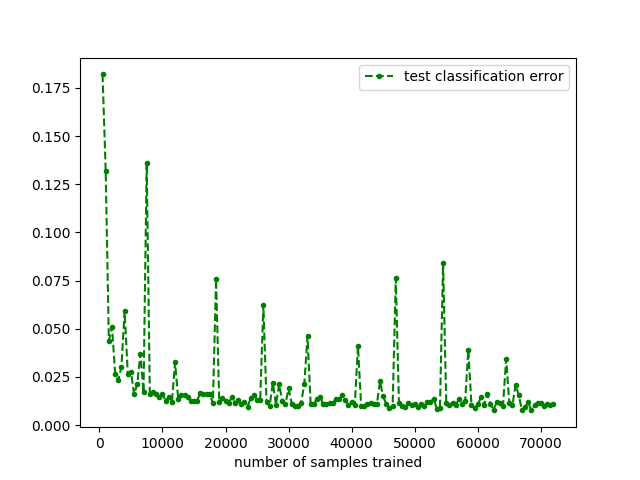
\includegraphics[scale=0.6]{Figure2.png}
\caption{Test classification error of simple LSTM model.}
\label{fig:test error}
\end{center}
\end{figure}

We also try a version of LSTM with a soft attention. 
\begin{align*}
\{h_1, h_2,..., h_T\} &= LSTM(\mathbf{X})\\
u_i &= v^{T}h_i\\
a_i &= SoftMax(u_i)\\
x_{weighted} &= \sum a_i x_i\\
\end{align*}
, where $v$ is a vector for attention computation. We use the weighted sum of words to predict the type of emotions since usually the emotion is borne in these words with emotion potential like "happy" and "congratulation". Here are some result of classification with attention weights. However, this assumption doesn't work well in the real, complicate world. But it seems to overfit on some words without considering the semantic information of the sentence. So we abandon this model and use a simple LSTM for emotion extraction.

\begin{table}[tbph]
\centering  % 表居中
\begin{tabular}{lccc}  % {lccc} 表示各列元素对齐方式,left-l,right-r,center-c
\hline
Sentence &Predicted emotion &True emotion\\ \hline  % \hline 在此行下面画一横线
I so pissed . Roger just stabbed me in the back . &joy &anger \\         % \\ 表示重新开始一行
I so frustrated . &sadness &sadness \\        % & 表示列的分隔线
It's so frustrating working with him . &love &anger\\ 
I was so frustrated , I stopped caring about the outcome . &fear &anger \\
I feeling pretty good right now . &joy &joy \\
I in a very good mood . &fear &joy \\
It feels so good taking a long vacation . &joy &joy \\
I got everything I ever wanted. I feel so blessed . &joy &joy \\ \hline
\end{tabular}
\caption{Predictions of some random sentences.}
\label{sentence}
\end{table}


















\newpage

\section*{References}

[1] Cho, K., Van Merriënboer, B., Bahdanau, D., \& Bengio, Y. (2014). On the properties of neural machine translation: Encoder-decoder approaches. arXiv preprint arXiv:1409.1259.


[2] Serban, I. V., Sankar, C., Germain, M., Zhang, S., Lin, Z., Subramanian, S., ... \& Mudumba, S. (2017). A Deep Reinforcement Learning Chatbot. arXiv preprint arXiv:1709.02349.

[3] Wang, W., Chen, L., Thirunarayan, K., \& Sheth, A. P. (2012, September). Harnessing twitter" big data" for automatic emotion identification. In Privacy, Security, Risk and Trust (PASSAT), 2012 International Conference on and 2012 International Confernece on Social Computing (SocialCom) (pp. 587-592). IEEE.

[4] Zhou, H., Huang, M., Zhang, T., Zhu, X., \& Liu, B. (2017). Emotional Chatting Machine: Emotional Conversation Generation with Internal and External Memory. arXiv preprint arXiv:1704.01074.

[5] Oriol Vinyals, Lukasz Kaiser, Terry Koo, Slav Petrov, Ilya Sutskever, Geoffrey Hinton (2014). Grammar as a Foreign Language. arXiv preprint arXiv:1412.7449. 
\end{document}
